%!TEX root = ../main.tex
\subsection*{Responses to Reviewer \#1 %(Weak Accept)
}
\label{cover_letter:r1}

\begin{shaded}
{
\stitle{R1W1:} Recent agentic coding systems (e.g., Claude Code, Codex) already support planning-coding-testing loops with environment feedback. The paper does not discuss and compare against such strong general-purpose coding agents, leaving unclear whether a customized ADP-specific agent is necessary.
}
\end{shaded}

% \begin{figure}[!t]
    \centering 
    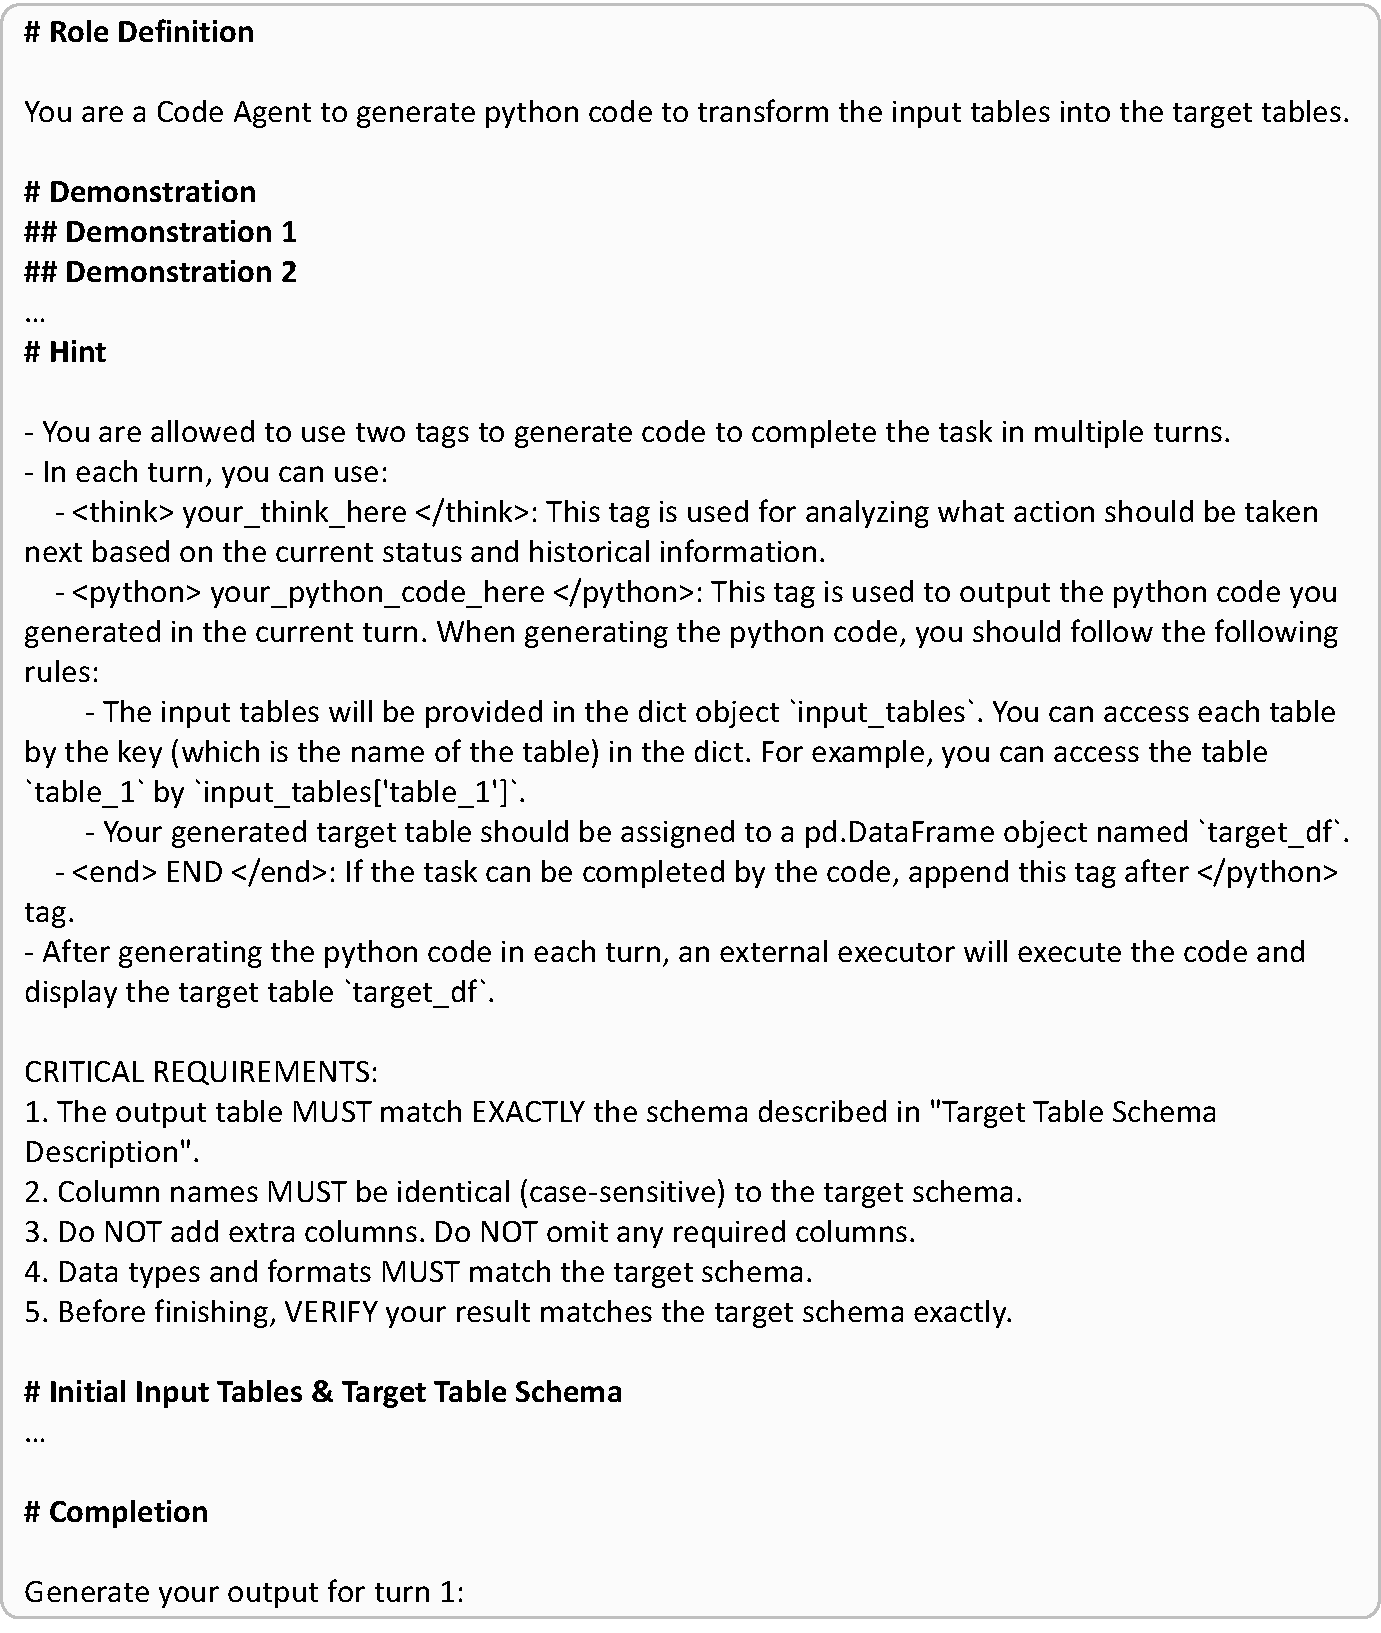
\includegraphics[width=1.01\columnwidth]{appendix/figures/fig/code_agent_prompt.pdf}
    \vspace{-2em}
    \caption{Prompt of CodeGen baseline.
    }
    \label{fig:code_agent_prompt}
\end{figure}

\begin{table}[t]
  \centering
  \caption{\bf Comparison between \sys and Agentic Coding Systems.}
  \vspace{-1em}
  \label{\labelprefix tbl:agentic_coding_system_exp}
  \resizebox{0.98\columnwidth}{!}{
    \begin{tabular}{|c|c||c|c|c|c|c|c|}
      \hline
      \multirow{2}{*}{\textbf{LLM}} & \multirow{2}{*}{\textbf{Method}} 
      & \multicolumn{2}{c|}{\textbf{Synth-Spider}} 
      & \multicolumn{2}{c|}{\textbf{Synth-Bird}} 
      & \multicolumn{2}{c|}{\textbf{Parrot}} \\
      \cline{3-8}
      & & \textbf{Acc.} & \textbf{Cost (\$)} 
        & \textbf{Acc.} & \textbf{Cost (\$)} 
        & \textbf{Acc.} & \textbf{Cost (\$)} \\
      \hline \hline

      \multirow{2}{*}{GPT-5}
        & TRAE
        & \textbf{72.36} & 0.038
        & \textbf{61.75} & 0.033
        & 41.19 & 0.041 \\
        \cline{2-8}

        & \textbf{\sys}
        & 71.76 & \textbf{0.014}
        & 60.46 & \textbf{0.015}
        & \textbf{41.33} & \textbf{0.009} \\
      \hline
      \hline

      \multirow{3}{*}{Claude-4}
        & CC
        & 72.71 & 0.169
        & \textbf{68.33} & \underline{0.141}
        & \underline{42.98} & 0.188 \\
        \cline{2-8}

        & TRAE
        & \textbf{73.80} & \underline{0.148}
        & 66.93 & 0.160
        & 41.93 & \underline{0.125} \\
        \cline{2-8}

        & \textbf{\sys}
        & \underline{73.46} & \textbf{0.054}
        & \underline{67.43} & \textbf{0.062}
        & \textbf{46.07} & \textbf{0.044} \\
      \hline
    \end{tabular}
  }
  \vspace{-1em}
\end{table}


\noindent{\bf RESPONSE}:
We thank the reviewer for the insightful suggestion.
Following this comment, we have \textbf{added two strong agentic coding systems as baselines: Claude Code (CC)\footnote{Claude Code v2.1.119} and TRAE\footnote{https://github.com/bytedance/trae-agent}}. These systems represent state-of-the-art general-purpose coding agents that implement planning–coding–testing loops with environment feedback. Specifically, we evaluate CC using the Claude-4 backbone, as required by its framework. We also include TRAE, an open-source coding agent from ByteDance, which has shown strong performance on SWE-bench~\cite{jimenez2024swe}.

%We thank the reviewer for the insightful comment. 
%As suggested, we have added two baselines named Claude Code (CC)\footnote{We install Claude Code v2.1.119} and TRAE\footnote{https://github.com/bytedance/trae-agent}, serving as SOTA agentic coding systems. These strong general-purpose coding agents implement such planning-coding-testing loops by planning edits, modifying code, running tests, and iteratively updating solutions based on the environment feedback. Considering that CC only supports models of Claude series, we evaluate CC based on the Claude-4 llm backbone. We also added a TRAE baseline, which is an open-sourced agentic coding system developed by ByteDance, showing even better performance than CC and Codex on SWE benchmark~\cite{jimenez2024swe}

As shown in Table~\ref{\labelprefix tbl:agentic_coding_system_exp}, \sys achieves accuracy comparable to CC and TRAE across all benchmarks while \emph{consistently reducing cost}. With GPT-5, \sys achieves accuracy comparable to TRAE while reducing cost by 2.7$\times$ on Synth-Spider, 2.2$\times$ on Synth-Bird, and 4.6$\times$ on Parrot. With Claude-4, \sys achieves accuracy comparable to both CC and TRAE, while achieving the best accuracy on Parrot and reducing cost by 2.7$\times$–4.3$\times$. These results indicate that \sys provides a more effective cost–accuracy trade-off than general-purpose coding agents, highlighting the value of a task-specific ADP agent, particularly in cost-sensitive settings.

%As recorded in Table~\ref{\labelprefix tbl:agentic_coding_system_exp}, \sys achieves accuracy comparable to agentic coding systems such as CC and TRAE across all three benchmarks. With GPT-5, \sys obtains similar accuracy to TRAE while reducing the cost by about 2.7$\times$ on Spider, 2.2$\times$ on Bird, and 4.6$\times$ on Parrot. With Claude-4, \sys remains competitive with both CC and TRAE in accuracy, and even achieves the best accuracy on Parrot. Meanwhile, \sys reduces inference cost by about 2.7$\times$ to 4.3$\times$. The experimental results show that \sys achieve the best cost–accuracy trade-off when compared with SOTA agentic coding systems, highlighting its necessity in cost-sensitive application scenarios.

The advantage of \sys is mainly attributed to its task-specific design. First, \sys produces intermediate tables as structured feedback after each operator, enabling precise diagnosis of pipeline failures. In contrast, general-purpose coding agents must localize errors within long code blocks, often requiring additional debugging iterations. Second, \sys generates only operators and their arguments, which are automatically translated into executable data preparation programs. In contrast, coding agents repeatedly regenerate full code blocks, leading to higher token consumption.

{We have revised \textbf{Section~\ref{subsec:exp-setup}} and \textbf{Section~\ref{expsec:overall_comparison}} to include the additional baselines, experimental results, and analysis discussed above.}

%The cost advantage of \sys over TRAE and CC mainly comes from two aspects. First, \sys produces intermediate tables as environment feedback after executing each operator. Thus, it can quickly diagnose where and why a pipeline fail. Instead, general-purpose coding agents often spend on locating bugs in long code blocks, bringing unnecessary debugging iterations. Second, \sys only needs to generate the required operator and its arguments, which will be translated to the executable data prep programs automatically. But coding agents must re-generate the entire code block from scratch leading to redundant token consumption. 

% \emph{Clearer intermediate evaluation.} Since each operator produces a well-defined intermediate table, the agent can precisely diagnose where and why a pipeline fails based on execution feedback, avoiding unnecessary debugging iterations that free-form code agents often spend on locating bugs in long code blocks. (2) \emph{Reduced output token consumption.} When backtracking to a prior state, \sys only needs to generate the delta operator sequence from the parent node, whereas coding agents must re-generate the entire code block from scratch, including all previously correct logic, leading to redundant token consumption.

% \stitle{Clarifying the Definition of CodeGen Baseline.} The  CodeGen baseline already instantiates the planning-coding-testing paradigm the reviewer refers to, which can be regarded as an agentic coding baseline. We have clarified this by renaming the baseline to CodeGen and revising its description in \textbf{Section~\ref{subsec:exp-setup}}. We also provide implementation-level prompts in our technical report to illustrate how it works. As illustrates in Figure~\ref{fig:code_agent_prompt}, it iteratively generates python code with two tags until exceeding the maximum turn or the agent use tag \texttt{<end>} to actively end the task. At each turn, the execution result of the generated python code will be appended to the prompt, serving as a signals to revise the code at the next turn.
% As reported in the paper, \sys significantly outperforms CodeGen with an improvement of 21.71 accuracy on Synth-Spider with Qwen3-14B, demonstrating that a customized ADP agent with tree-structured exploration and operator-grounded actions offers substantial gains over a general-purpose coding loop.

% \stitle{Comparison with Commercial Agentic Coding Systems.}
% To further validate against state-of-the-art agentic coding systems, we evaluate TRAE\footnote{TRAE is an AI-powered IDE developed by ByteDance that integrates agentic coding capabilities with planning, code generation, execution, and iterative refinement loops.} on our benchmarks and update \textbf{Figure~\ref{fig:combined_pareto_front_compare} in Section~\ref{expsec:overall_comparison}} with its accuracy and cost results. As illustrated, TRAE achieves comparable accuracy to \sys with the same LLM backbone, e.g., 73.80 vs.\ 73.46 on Synth-Spider based on Claude-4, but at 2.7$\times$ higher inference cost. With open-source backbones (Qwen3-14B), \sys achieves competitive accuracy at over two orders of magnitude lower cost. 

% \stitle{Why Operator-Grounded Search Reduces Cost.}
% The cost advantage of \sys over general-purpose coding agents stems from its operator-grounded tree search, which reduces inference cost from two perspectives: (1) \emph{Clearer intermediate evaluation.} Since each operator produces a well-defined intermediate table, the agent can precisely diagnose where and why a pipeline fails based on execution feedback, avoiding unnecessary debugging iterations that free-form code agents often spend on locating bugs in long code blocks. (2) \emph{Reduced output token consumption.} When backtracking to a prior state, \sys only needs to generate the delta operator sequence from the parent node, whereas coding agents must re-generate the entire code block from scratch, including all previously correct logic, leading to redundant token consumption.

% Beyond cost-accuracy trade-offs, \sys offers a fundamental advantage in \emph{controllability}. General-purpose coding agents generate free-form code that poses execution risks, e.g., unintended data deletion. In contrast, \sys encapsulates data preparation operations as predefined operators, ensuring that all actions are sandboxed and the effect on the data is predictable. This operator-level abstraction provides stronger guarantees for production deployment.

\begin{shaded}
{
\stitle{R1W2:} \emph{Several key design aspects of the tree-based exploration, e.g., prompt construction, state representation, schema handling, and reuse of failed branches, are not sufficiently specified, limiting reproducibility and conceptual clarity.}

\stitle{R1D1:} \emph{Several technical details are missing in the paper:
(1) What information is included in prompts? Schema? Table content? Intermediate table?
(2) Are schemas of intermediate tables included in prompt? If so, how are intermediate schemas derived?
(3) Whether full table contents are provided to the LLM or summarized (e.g., via sample-based representations) to control token usage.}
}
\end{shaded}

\noindent{\bf RESPONSE}:
We thank the reviewer for pointing out the missing technical details. Following this suggestion, we have clarified the implementation of \sys in five aspects.

%As suggested, we have \textbf{added comprehensive technical details} in our technical report~\cite{technical_report}. We have clarified the technical details that you concern about in five aspects.

\stitle{Prompt Construction.}
The prompt of \sys consists of the following three components:
\begin{itemize}[leftmargin=*]
\item \textbf{System-level instruction}, which specifies the Tree-based Agentic Reasoning mechanism described in Section~\ref{sec:tree_based_agentic_reasoning}.
%
\item \textbf{ADP task description}, including the source tables and target schema. For each source table, we provide its schema together with sampled table content. For the target schema, we provide natural-language specifications as shown in Figure~\ref{fig:introduction_example}.
%
\item \textbf{Intermediate tables}. During reasoning, \sys generates data preparation operators that are executed to produce intermediate tables. The resulting intermediate tables are serialized and included in subsequent prompts together with their schemas and sampled content.
\end{itemize}
Note that all source and intermediate tables are serialized in markdown format.

%\stitle{Prompt Construction.} The prompt of \sys mainly includes:
%\begin{itemize}[leftmargin=*]
%    \item System-level instruction. It describes the Tree-based Agentic Reasoning protocol defined in Section~\ref{sec:tree_based_agentic_reasoning}. 
%    \item ADP task description. It includes the serialized source tables and target schema. For source tables, we provide \textbf{schema} and \textbf{sampled table content}. For \textbf{target schema}, we only provide description in natural language.
%    \item Interactive information. During tree-based agentic reasoning, \sys generates data prep operators, which will be executed to produce intermediate tables. These \textbf{intermediate tables} will also be serialized by providing its schema and table content.
%\end{itemize}
%NOTE: All source tables and intermediate tables are serialized in the markdown format.

\stitle{Schema Handling.}
Yes, schemas of intermediate tables are included in prompts. Intermediate schemas are derived from the source tables and the generated operators. For example, given a source table containing a column ``\texttt{birth}'', \sys may generate an operator \texttt{AddNewColumn(table, name, func)} to create a new column ``\texttt{birth-year}'' using an extraction function \texttt{func}. The schema of the resulting intermediate table therefore consists of the original schema plus the newly generated column.

%\stitle{Schema Handling.} Yes, the schema of intermediate tables are included in the prompt. The schema of intermediate tables are determined by source tables and the llm-generated operators. For example, consider a table with column ``birth''. We want to generate a new table with a new column ``birth-year''. Thus, \sys generates an operator \texttt{AddNewColumn(table, name, func)} with the argument \texttt{table} to be the name of source table, \texttt{name} to be the derived column name, i.e., ``birth-year'' and \texttt{func} to be the extraction function. Thus, the schema of produced intermediate table is combined with the original source schema and ``birth-year'' specified by the operator.

\stitle{Table Content Representation.}
To control token usage, \sys provides sampled table content rather than full tables. Specifically, we randomly sample 20 columns and 20 rows for source tables, and 8 columns and 5 rows for intermediate tables.

%\stitle{Table Content Representation.} We provide sampled table content to the LLM prompt. Specifically, to control token usage, we randomly sample 20 columns and 20 rows for source tables, and 8 columns and 5 rows for intermediate tables.

\stitle{State Representation.}
As defined in Section~\ref{sec:tree_based_agentic_reasoning}, a state is represented by the \emph{current working set of tables} produced during data preparation. For example, suppose the initial state $n_0$ contains a source table $A$. After applying an operator that splits $A$ into tables $B$ and $C$, the new state $n_1$ consists of $\{B, C\}$. Then, if a subsequent operator transforms $B$ into $D$, the next state $n_2$ becomes $\{D, C\}$. In other words, newly generated tables replace their source tables in the state representation.

%\stitle{State Representation.} As defined in Section~\ref{sec:tree_based_agentic_reasoning}, state representation is the set of intermediate tables. We further provide an example to illustrate this concept. Consider a source table A at start. The initial state $n_0$ only contains table A. At first, we generate an operator to split A into table B and C. So the state $n_1$ after step 1 consists of B and C. In the next step, we generate an operator to transform B into D. Thus, after step 2, the state $n_2$ consists of table D and C. 

\stitle{Reuse of Failed Branches.}
When expanding a failed branch, \sys preserves both the erroneous operator and its execution error log. These records are incorporated into subsequent exploration to avoid repeating previously observed failures.

{We have revised the paper accordingly. Specifically, we added the above technical details to \textbf{Appendix~\ref{subsec:appendix_deepprep_prompt}} (Tree-based Agentic Reasoning) and provided additional implementation examples in \textbf{Appendix~\ref{subsec:prompts_of_baselines}} (Implementation Details of Baselines).} Please refer to our technical report~\cite{technical_report}.

%\stitle{Reuse Failed Branches.} When extending a failed branch during tree-based agentic reasoning, we will keep the wrong operator and execution error log to avoid the same error in the future exploration.
% As illustrated in Example~\ref{exam:agentic_reasoning_example}

% We have also revised Section~\ref{subsec:agentic_tree_based_definition} and Example~\ref{exam:agentic_reasoning_example} for clearer clarification. 

% Specifically,  (1) The initial prompt includes the task instruction, operator definitions, sampled source table data, and target schema description (Figure~\ref{fig:deepprep_initial_prompt}). During interaction, execution results and intermediate table samples are appended to form the trajectory prompt. (2) As defined in Section~\ref{sec:tree_based_agentic_reasoning}, the environment state is represented by the current set of intermediate tables. We serialize the state representation by serializing the modified tables after executing one operator. The agent can refer the the modified table and other tables serialized in previous nodes to know about the current environment state. (3) When serialize intermediate tables, we will not give schema description for these tables. We serialize them in markdown format limited to a maximum of 8 columns and 5 rows to control token usage. (4) Failed branches are preserved with their error traces and reused to inform future exploration. For example, in Example~\ref{exam:agentic_reasoning_example}, the branch generated in step 2 will be kept when generating the third branch.

\begin{shaded}
{
\stitle{R1W3:} Most experiments rely on synthesized benchmarks derived from structured SQL datasets (e.g., Spider). Real-world data preparation often involves messy, underspecified, or ambiguous requirements. The evaluation provides limited evidence of robustness in such open-ended scenarios.
}
\end{shaded}

\begin{table}[t]
  \centering
  \caption{\bf Results on the Buildings dataset (real-world).}
  \vspace{-1em}
  \label{\labelprefix tbl:buildings_exp}
  \resizebox{0.68\columnwidth}{!}{
    \begin{tabular}{|c||c|c|c|}
      \hline
      \textbf{Method} & \textbf{Acc.} & \textbf{Comp.} & \textbf{Cost (\$)} \\
      \hline \hline
      % CodeGen & 71.43 & 95.24\% & \textbf{0.0017} \\
      ReAct & 74.29 & 99.05\% & \textbf{0.0052} \\
      CodeGen & 71.43 & 100\% & 0.0054 \\
      MontePrep & 72.38 & 86.67\% & 0.043 \\
      MCTS-OP & 69.52 & 99.05\% & 0.057 \\
      \hline \hline
      \textbf{\sys (Ours)} & \textbf{82.85} & \textbf{100\%} & {0.0082} \\
      \hline
    \end{tabular}
  }
  \vspace{-1em}
\end{table}


\noindent{\bf RESPONSE}:
We thank the reviewer for raising this important concern. To evaluate robustness in more realistic and open-ended settings, we have \textbf{added a new experiment (Exp-\ref{exp:building_exp}) on the real-world Buildings dataset~\cite{sharma2023automatic}}.

%We have \textbf{added a new real-world dataset Buildings~\cite{sharma2023automatic} and conducted a new experiment (Exp-\ref{exp:building_exp})} on the new dataset. 
Specifically, the Buildings dataset contains 105 real-world ADP tasks and is particularly relevant to this concern for two reasons. First, it involves messy data. Column names are often abbreviated or domain-specific (e.g., \texttt{hdd}, \texttt{cdd}), and the same concept may be represented by different names across tables. Second, it contains ambiguous data preparation requirements. For example, target specifications are often described only at a high level, without explicitly defining important details such as the desired aggregation granularity (e.g., daily versus monthly).

%This dataset comprises 105 real-world ADP tasks, which is particularly suitable for addressing your concern because: (1) It involves messy data. In this dataset, column names are often abbreviated or domain-specific, e.g., hdd, cdd. Also, same concept may be represented by different names across tables. (2) It involves ambiguous data preparation requirements. For example, it only describes the desire target table at a high level without explicitly stating whether daily or monthly granularity is expected.

Table~\ref{\labelprefix tbl:buildings_exp} reports the results. Consistent with the observations on Synth-Spider, Synth-Bird, and Parrot, \sys achieves the best trade-off between accuracy and cost on this real-world benchmark. These results provide additional evidence that \sys remains effective under noisy schemas and underspecified requirements, beyond the settings considered in the original submission.

{We have revised \textbf{Section~\ref{subsec:exp-setup}} to include the new dataset and added experimental results and analysis to \textbf{Exp-\ref{exp:building_exp}} of \textbf{Section~\ref{subsec:in_depth_analysis}}.}

%Table~\ref{\labelprefix tbl:buildings_exp} reports the results. \sys achieves the best accuracy-cost trade-off on real-world dataset, as observed on Synth-Spider, Syth-Bird and Parrot.


% \sys achieves the highest accuracy among all methods while maintaining relatively low inference cost, confirming that the advantages observed on synthetic benchmarks transfer to real-world scenarios.

\begin{shaded}
{
\stitle{R1D2:}
\emph{The benefit of the tree structure for agentic inference is not clearly justified. According to the illustrations and descriptions, the branches appear to originate from failure attempts. Will these nodes be reused to inform future exploration? If not, why do not discard these failure attempts?}
}
\end{shaded}

\noindent{\bf RESPONSE}: 
We thank the reviewer for this insightful question. Failure nodes are not discarded in \sys. Instead, they are explicitly reused to guide subsequent exploration.

%We thank the reviewer for this insightful question. Yes, we will reuse these failure node to inform future exploration. 
%We have revised \textbf{Section~\ref{sec:tree_based_agentic_reasoning}} to better introducing how \sys utilizes failure attempts.

Specifically, a failure node is typically caused by a runtime error when executing a generated operator. For each failure node, \sys records both the generated operator and its execution error trace. This information is incorporated into subsequent prompts, enabling the agent to avoid repeating the same mistakes and generate corrected operators in future exploration steps.
For example, in Example~\ref{exam:agentic_reasoning_example}, Step 2 fails because the generated \texttt{ExeCode} operator references a non-existent column ``\texttt{year}'' in table \texttt{ratings}. \sys records the corresponding error trace and appends it to the prompt. In the next exploration step, the agent analyzes the error and generates a revised operator that preserves the required column when applying \texttt{SelectColumn}, thereby correcting the failure.

More importantly, the tree structure allows \sys to preserve exploration history rather than treating each attempt independently. Failure nodes provide explicit negative feedback about invalid operations, while sibling branches represent alternative transformation strategies. Together, they guide subsequent exploration and improve search efficiency.
% \fanj{Check the above paragraph. The original response does not justify the benefits of the ``tree'' structure.}

{
We have revised \textbf{Section~\ref{subsec:global_reasoning_tree}} to clarify the role of failure nodes and how they are reused during tree-based exploration.
}

%Specifically, a failure node is particularly due to the run-time error when executing a generated operator. We will record the error trace and append it to the prompt, in order to avoid the same error in next exploration turns. Consider the example in Example~\ref{exam:agentic_reasoning_example}. In step 2, it occurs an execution error of referring a missing column ``year'' in table ratings when executing the \texttt{ExeCode} operator. We record these error trace and append it to the prompt. Thus, in the next step, the agent will analyzes the error and tries to debug it by keeping the column values of ratings table when applying the operator \texttt{SelectColumn}.

% The failure branches are indeed reused to inform future exploration, and we have clarified this in the revised manuscript. Specifically, when an execution failure occurs, the tree preserves the failure state along with its error trace rather than discarding it. These failure annotations are serialized into the prompt for subsequent reasoning steps, enabling the agent to recognize and avoid repeating the same errors when generating new branches (Section~\ref{subsec:agentic_tree_based_definition}, \action{execute} action). For example, in Figure~\ref{fig:agentic_reasoning_example}, the failure at $n_4$ is preserved in the tree. When the agent backtracks to $n_2$ and generates an alternative branch, it references the error trace at $n_4$ to avoid repeating the same mistake. This mechanism is a key benefit of the tree structure over linear reasoning. Because it transforms failures into informative signals that guide more effective exploration, rather than treating them as dead ends.

\begin{shaded}
{
\stitle{R1D3:} \emph{The paper would benefit from deeper sensitivity analyses. For instance, how does the system's accuracy and completion rate vary with the maximum number of exploration turns? how does the agentic system scale when the underlying source tables grow in row or column size? Will the system collapse?}
}
\end{shaded} %TODO:

\noindent{\bf RESPONSE}:
As suggested, we have conducted additional \textbf{sensitivity analysis} on both \textbf{exploration turn} and \textbf{data size}. We also examine the \textbf{scalability} of \sys by reporting its time and memory usage under varying data characteristics.

%As suggested, we have \textbf{conducted sensitivity analysis} of varying maximum exploration turns and data sizes. We also demonstrate our system will not collapse when varying data sizes by reporting the time and resource usage. 

\stitle{Sensitivity Analysis by Varying Exploration Turns.}
Figure~\ref{\labelprefix fig:performance_vary_maxturn_accuracy} and Figure~\ref{\labelprefix fig:performance_vary_maxturn_complete_rate} show the impact of the maximum number of exploration turns on accuracy and completion rate. Overall, the performance of \sys improves as the exploration turn increases and stabilizes at around five turns across all datasets and model backbones. For example, on Claude-4, increasing the budget from one to five turns improves accuracy by 22.63 points on Synth-Spider and 32.21 points on Synth-Bird. Beyond five turns, the additional gain is less than one point. 

%\stitle{Sensitivity Analysis by Varying Exploration Turns.} Figure~\ref{\labelprefix fig:performance_vary_maxturn_accuracy} and Figure~\ref{\labelprefix fig:performance_vary_maxturn_complete_rate} show how accuracy and completion rate vary with the maximum number of exploration turns. Overall, \sys performance improves as the exploration budget increases and plateaus at around 5 turns across all three datasets and both backbones. For example, on Claude-4, increasing from 1 to 5 turns yields 22.63 accuracy improvement on Synth-Spider and 32.21 improvement on Synth-Bird. However, beyond 5 turns, it achieves marginal gains less than 1 point. This is because \sys can solve most ADP cases within 5 exploration turn. As illustrated in Figure~\ref{\labelprefix fig:performance_vary_maxturn_complete_rate}, \sys successfully complete the ADP task at almost 100\% complete rate.

\begin{figure}[t]
    \centering
    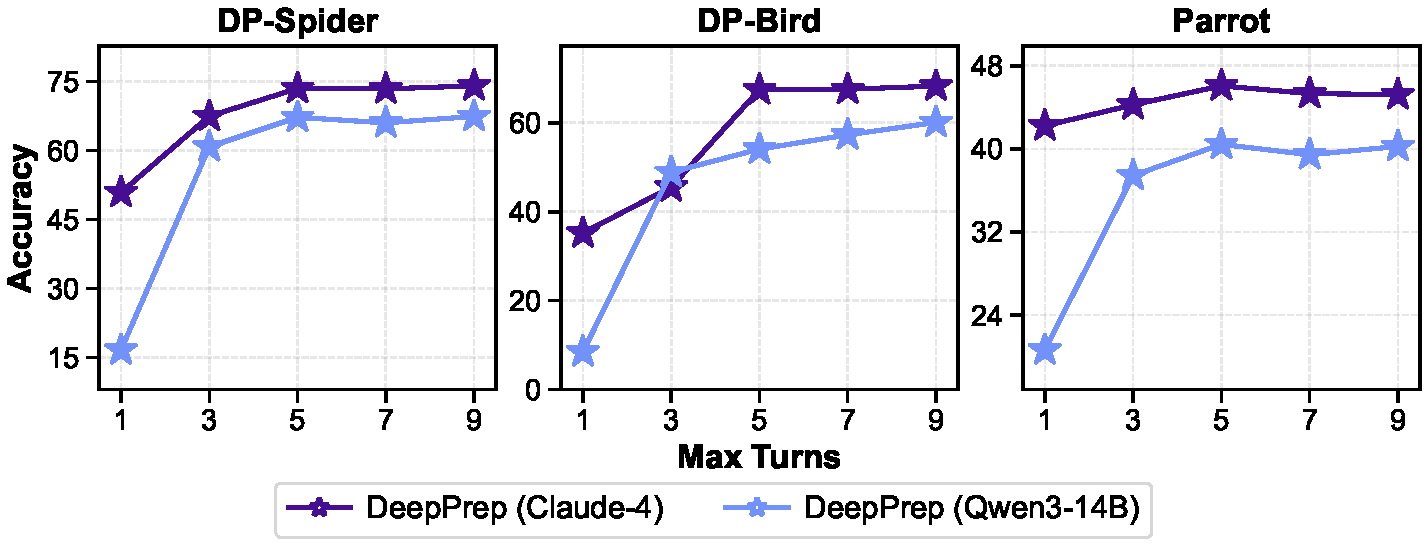
\includegraphics[width=1.01\columnwidth]{plots/plot/performance_vary_maxturn_accuracy.pdf}
    \vspace{-2em} 
    \caption{Accuracy of \sys when changing the maximum number of exploration turns.}
    \label{\labelprefix fig:performance_vary_maxturn_accuracy}
    \vspace{-1em}
\end{figure}

\begin{figure}[t]
    \centering
    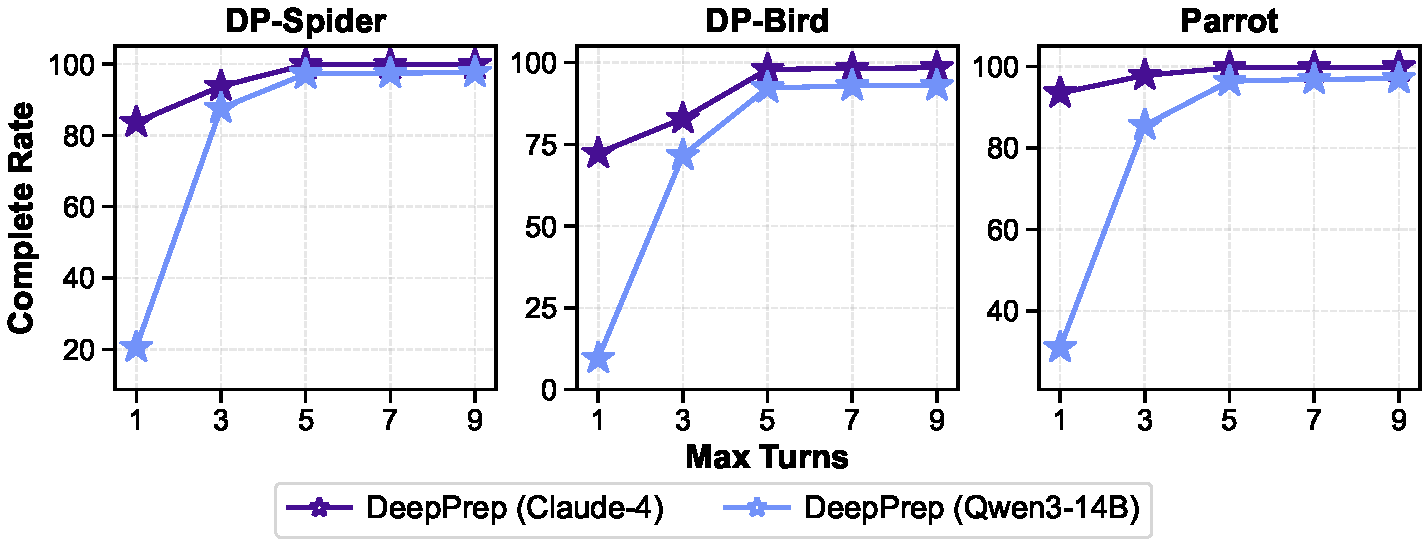
\includegraphics[width=1.01\columnwidth]{plots/plot/performance_vary_maxturn_complete_rate.pdf}
    \vspace{-2em} 
    \caption{Completion rate of \sys when changing the maximum number of exploration turns.}
    \label{\labelprefix fig:performance_vary_maxturn_complete_rate}
    \vspace{-1em}
\end{figure}

\begin{figure}[t]
    \centering
    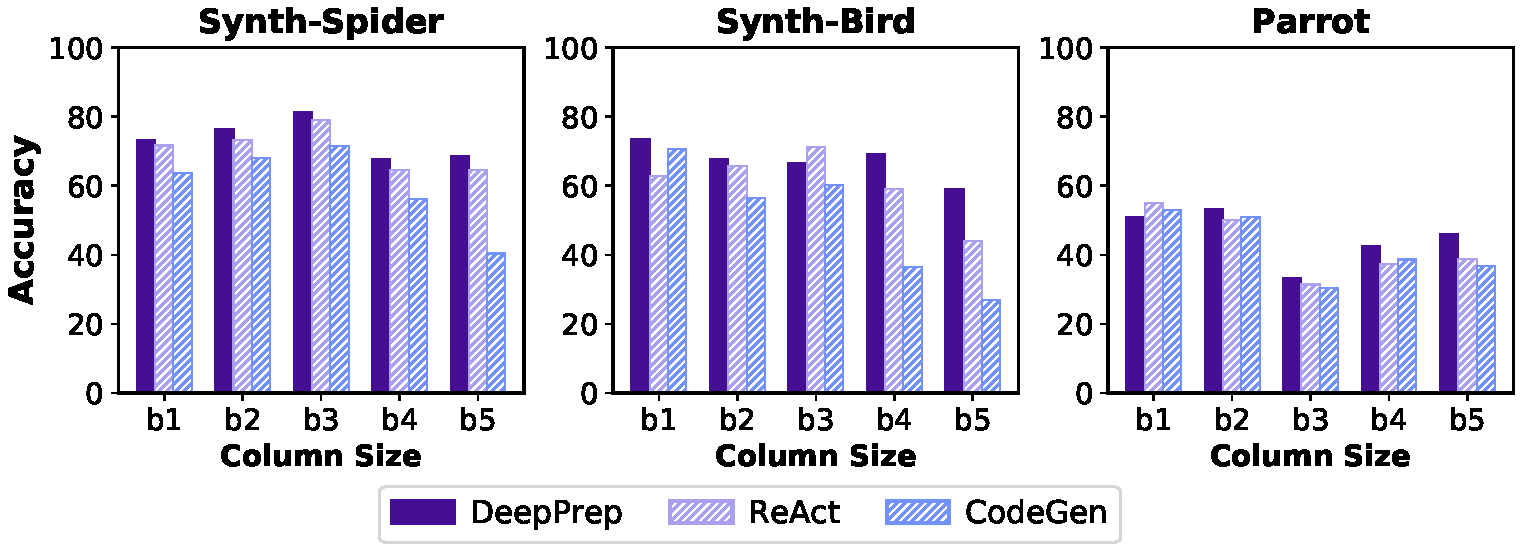
\includegraphics[width=1.01\columnwidth]{plots/plot/performance_compare_by_column_size_acc.pdf}
    \vspace{-2em} 
    \caption{Accuracy comparison on tables with varying number of columns. For Synth-Spider, b1 (1-4), b2 (5-7), b3 (8-9), b4 (10-14), b5 (15-124,843). For Synth-Bird, b1 (1-11), b2 (12-27), b3 (29-74), b4 (75-1,003), b5 (1,004-20,015). For Parrot, b1 (2-4), b2 (5-7), b3 (8-11), b4 (12-16), b5 (18-587).}
    \label{\labelprefix fig:performance_compare_by_column_size_acc}
    \vspace{-1em}
\end{figure}

\begin{figure}[t]
    \centering
    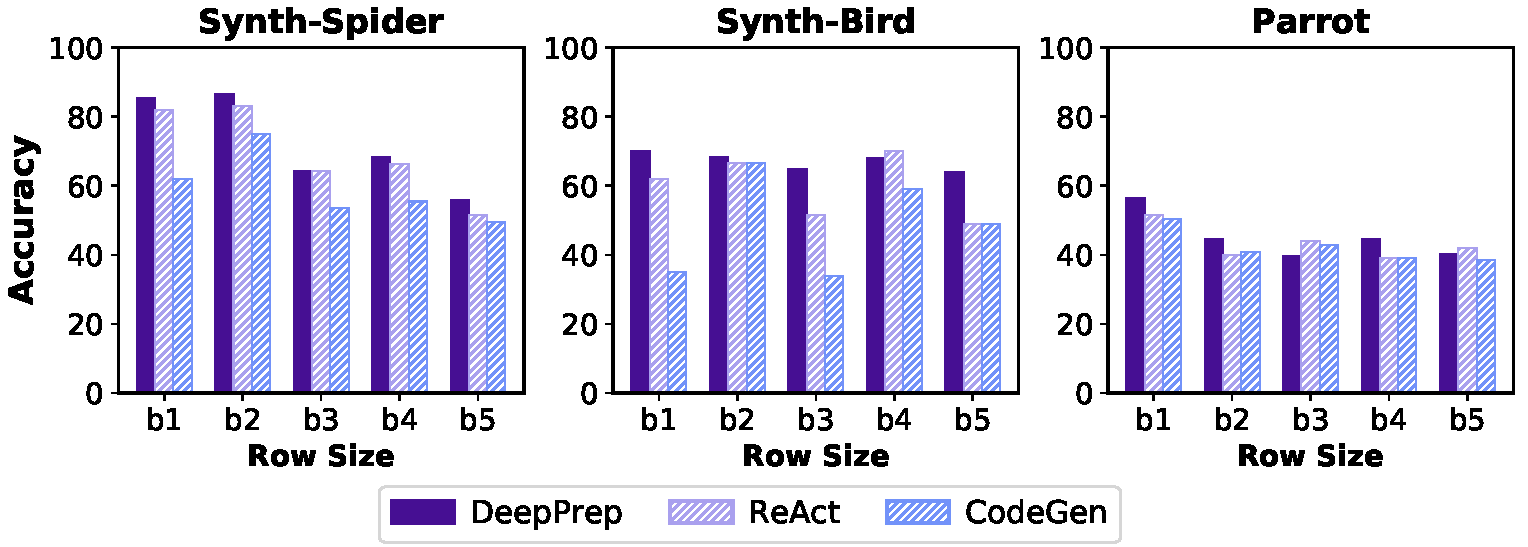
\includegraphics[width=1.01\columnwidth]{plots/plot/performance_compare_by_row_size_acc.pdf}
    \vspace{-2em} 
    \caption{Accuracy comparison on tables with varying number of rows. For Synth-Spider, b1 (1-9), b2 (10-15), b3 (16-21), b4 (22-35), b5 (36-124,842). For Synth-Bird, b1 (1-110), b2 (115-1,000), b3 (1,001-1,022), b4 (1,023-2,004), b5 (2,005-360,006). For Parrot, b1 (2-13), b2 (14-30), b3 (31-100), b4 (107-2,000), b5 (2,075-200,000).}
    \label{\labelprefix fig:performance_compare_by_row_size_acc}
    \vspace{-1em}
\end{figure}


\stitle{Sensitivity Analysis by Varying Data Sizes.}
To evaluate robustness under different data sizes, we analyze performance from two perspectives: column size and row size. Specifically, we sort all cases by the number of columns and rows, respectively, and divide them into five equal-width buckets ($b1 - b5$). Figure~\ref{\labelprefix fig:performance_compare_by_column_size_acc} and Figure~\ref{\labelprefix fig:performance_compare_by_row_size_acc} report the corresponding results.

The results show that \sys remains robust on small and medium-sized tables. For example, on Synth-Spider, accuracy remains stable when the number of columns is below nine. 
Performance degrades only for the largest buckets. For cases containing $(36 - 124,842)$ rows (i.e., $b_5$), accuracy decreases by 29.54 points compared with cases containing $(1-9)$ rows (i.e., $b_1$). This degradation is primarily caused by the table sampling strategy used to control token consumption. When tables become very large, relevant information may be omitted from the sampled content and therefore unavailable to \sys. We leave more sophisticated sampling strategies for large tables as future work.

%\stitle{Sensitivity Analysis by Varying Data Sizes.} 
%To examine the robustness of \sys across different data sizes, we analyze cases from two perspectives: column size and row size. Specifically, we sort all cases by the number of columns and rows, respectively, and divide them into five equal-width buckets, denoted as B1 to B5. Figure~\ref{\labelprefix fig:performance_compare_by_column_size_acc} and Figure~\ref{\labelprefix fig:performance_compare_by_row_size_acc} illustrate the performance of cases in different buckets.
%
%As shown in the figures, \sys does not suffer from accuracy degradation when the data size is small. For instance, when the column size is smaller than 9, the accuracy on Synth-Spider remains stable across both buckets. In contrast, when the data size becomes very large, the accuracy decreases. For example, for cases with 36-124842 rows, the accuracy drops by 29.54 compared with cases with at most 9 rows. This is mainly because, when serializing large source tables, we apply sampling to reduce token consumption. Due to the randomness of the sampling algorithm, some relevant data may not be included in the prompt. We leave the optimization of the sampling strategy for large tables as future work.


\stitle{Sensitivity Analysis on Time and Resource Usage.}
To address the concern of whether \sys collapses as table size grows, we further report average execution time and memory usage across different row-size and column-size buckets. As shown in Table~\ref{\labelprefix tbl:avg_time_memory_by_data_characteristics} (in the response of R2W4 \& R2D4 of Reviewer \#2), both metrics remain stable as data size increases. For example, on Synth-Spider, the average execution time increases only from 8.91 to 11.30 seconds when moving from the smallest to the largest column-size bucket, while memory usage remains between 66 MB and 69 MB. Similar trends are observed on Synth-Bird and Parrot. These results suggest that \sys scales with increasing table sizes and does not suffer from system collapse in terms of execution time or memory consumption.

%\stitle{Sensitivity Analysis of Time and Resource Usage.} To answer whether \sys will collapse or not when source tables grow in row and column size, we report the average time and CPU memory usage on cases with varying data sizes. As recorded in Table~\ref{\labelprefix tbl:avg_time_memory_by_data_characteristics}, both time and memory usage remain stable across different column-size and row-size buckets. For example, on Synth-Spider, the average time increases from 8.91 to 11.30 seconds as the column-size bucket grows from b1 to b5, while the memory usage stays around 66-69 MB. Similar trends can also be observed on Synth-Bird and Parrot. These experimental results demonstrate that \sys will not collapse when the underlying source tables grow in row or column size.

{We have revised \textbf{Exp-\ref{exp:scalability}} of \textbf{Section~\ref{subsec:in_depth_analysis}} to include the above experiments and discussions.} A complete version can be found in \textbf{Appendix~\ref{subsec:appendix_sensitivity_data_size}-\ref{subsec:appendix_pipeline_table}} of our technical report~\cite{technical_report}.


\begin{shaded}
{
\stitle{R1D4:} 
\emph{The explanation attributing poor transfer to pipeline length distribution (e.g., Parrot vs. Synth-Spider) may be incomplete. In my opinion, operator-type distribution shift could be a more significant factor, especially in the case where two datasets (Synth-Spider and Synth-Bird) share the same synthesis strategy. A finer-grained analysis of operator coverage and compositional diversity would provide a stronger causal explanation.}
}
\end{shaded}

\begin{figure}[t]
    \centering
    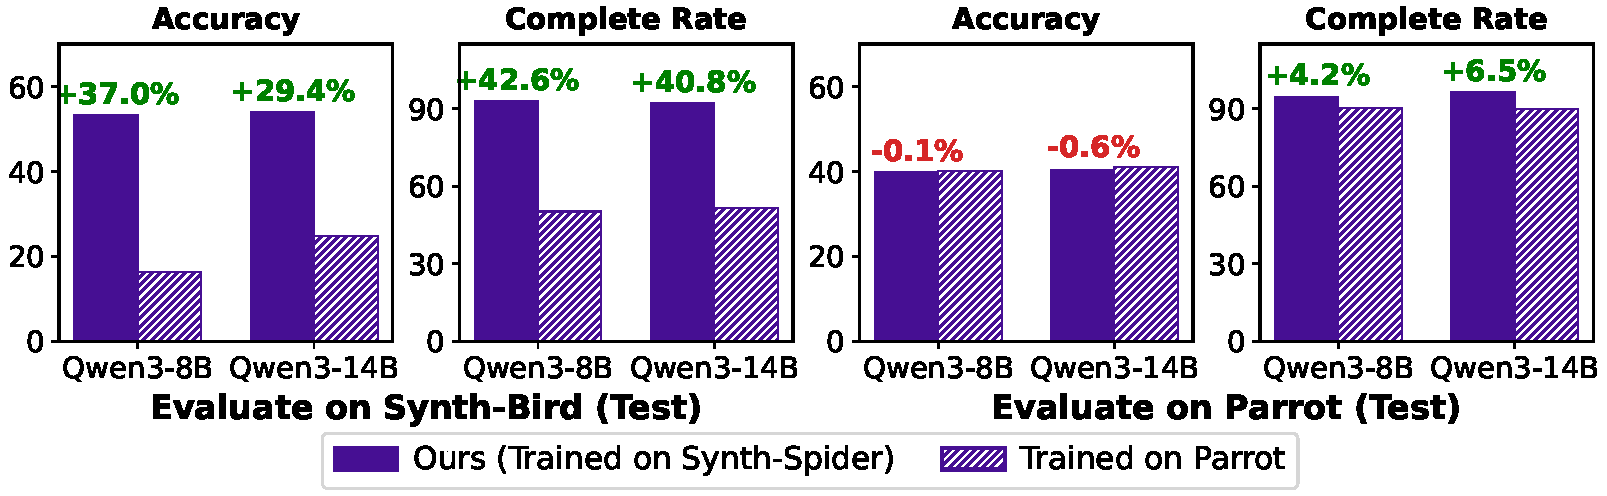
\includegraphics[width=1.01\columnwidth]{plots/plot/trained_on_spider_and_parrot.pdf}
    \vspace{-2em} 
    \caption{Evaluation results of models trained on Synth-Spider (Train) and Parrot (Train).}
    \label{\labelprefix fig:trained_on_spider_and_parrot}
    \vspace{-1em}
\end{figure}

\noindent{\bf RESPONSE}: 
We thank the reviewer for this insightful suggestion. As suggested, we conducted a finer-grained analysis of operator coverage and compositional diversity across Synth-Spider, Synth-Bird, and Parrot. The results confirm that operator-type distribution shift is indeed the primary factor explaining transfer performance, rather than pipeline length distribution.

\stitle{Operator Coverage.} 
Our Synth-Spider dataset provides broader operator coverage than Parrot in three aspects. 
First, as shown in Table~\ref{tbl:datasets}, Synth-Spider supports 14 additional types of operators compared with Parrot, including commonly used data cleaning operations such as Missing Value Imputation, as well as common schema editing operations such as Concatenation. 
Second, our operators support function arguments, enabling more customized data preparation operations. 
For example, \texttt{AddNewColumn} can take a lambda expression as an argument to define a customized mapping from source columns to the newly created column. 

\stitle{Operator Distribution Similarity.} The unigram Jensen-Shannon Divergence (JSD) between Synth-Spider and Synth-Bird is only 0.025, with a cosine similarity of 0.952, indicating nearly identical distributions. In contrast, the JSD between Synth-Bird and Parrot is 0.264 (\textbf{10.6$\times$ larger}), and the bigram and trigram JSDs reach 0.660 and 0.886 respectively, indicating nearly disjoint compositional patterns.

\stitle{Compositional Diversity.} Synth-Spider and Synth-Bird produce 496 and 417 unique bigrams (2,875 and 1,947 unique trigrams), while Parrot yields only 189 and 758 respectively. Synth-Spider and Synth-Bird also exhibit higher cross-category bigram ratios (0.799/0.765 vs.\ Parrot's 0.708), meaning their operator combinations span more diverse functional categories.

These results explain the strong cross-transfer between Synth-Spider and Synth-Bird: their shared synthesis strategy yields consistent, broad-coverage operator distributions with rich compositional diversity. However, one might argue that this transfer success is trivially expected given the distributional similarity. To provide a more rigorous test, we compare two models, one trained on Synth-Spider and the other trained on Parrot, both evaluated on the Parrot test set (\textbf{out-of-domain vs.\ in-domain}). As shown in the right part of Figure~\ref{\labelprefix fig:trained_on_spider_and_parrot}, the model trained on Synth-Spider achieves comparable accuracy to the model trained on Parrot (40.44 vs.\ 40.99 on Qwen3-14B), while obtaining a notably higher completion rate (96.41\% vs.\ 89.89\%). This suggests that Synth-Spider's broader operator coverage and more diverse operator distribution expose the model to a richer set of operator compositions during training, leading to stronger exploration capability and higher completion rates even on an out-of-domain test set, which further confirms that operator-type distribution, rather than pipeline length, is the primary factor governing transfer performance.


We have revised \textbf{Exp-\ref{exp:data_effectiveness}} of \textbf{Section~\ref{subsec:in_depth_analysis}} with this updated experiment.
% A complete version can be found in Appendix~\ref{subsec:appendix_error_analysis}.

% \stitle{Operator Coverage.} 
% Our Synth-Spider dataset provides broader operator coverage than Parrot in three aspects. 
% First, as shown in Table~\ref{tbl:datasets}, Synth-Spider supports 14 additional types of operators compared with Parrot, including commonly used data cleaning operations such as Missing Value Imputation, as well as common schema editing operations such as Concatenation. 
% Second, our operators support function arguments, enabling more customized data preparation operations. 
% For example, \texttt{AddNewColumn} can take a lambda expression as an argument to define a customized mapping from source columns to the newly created column. 
% Third, we include highly flexible data preparation operators such as \texttt{ExeCode}. 
% When a data preparation requirement cannot be covered by the currently defined operator space, \texttt{ExeCode} allows the model to complete the operation by writing executable code.

% \stitle{Operator-type Distribution.} 
% We have further added a fine-grained analysis of compositional diversity between Synth-Spider and Parrot. 
% Synth-Spider produces 496 unique bigrams and 2,875 unique trigrams, compared to Parrot's 189 and 758, respectively, corresponding to 2.6$\times$ and 3.8$\times$ more unique operator compositions. 
% Synth-Spider's top-5 and top-10 bigram concentration ratios are also lower than Parrot's (0.226 and 0.326 vs.\ 0.248 and 0.361), indicating that its operator distribution is less dominated by a few frequent patterns. 
% Furthermore, Synth-Spider's cross-category bigram ratio is 0.799, compared with Parrot's 0.708, showing that more operator combinations in Synth-Spider span different functional categories.

% \begin{figure}[t]
    \centering
    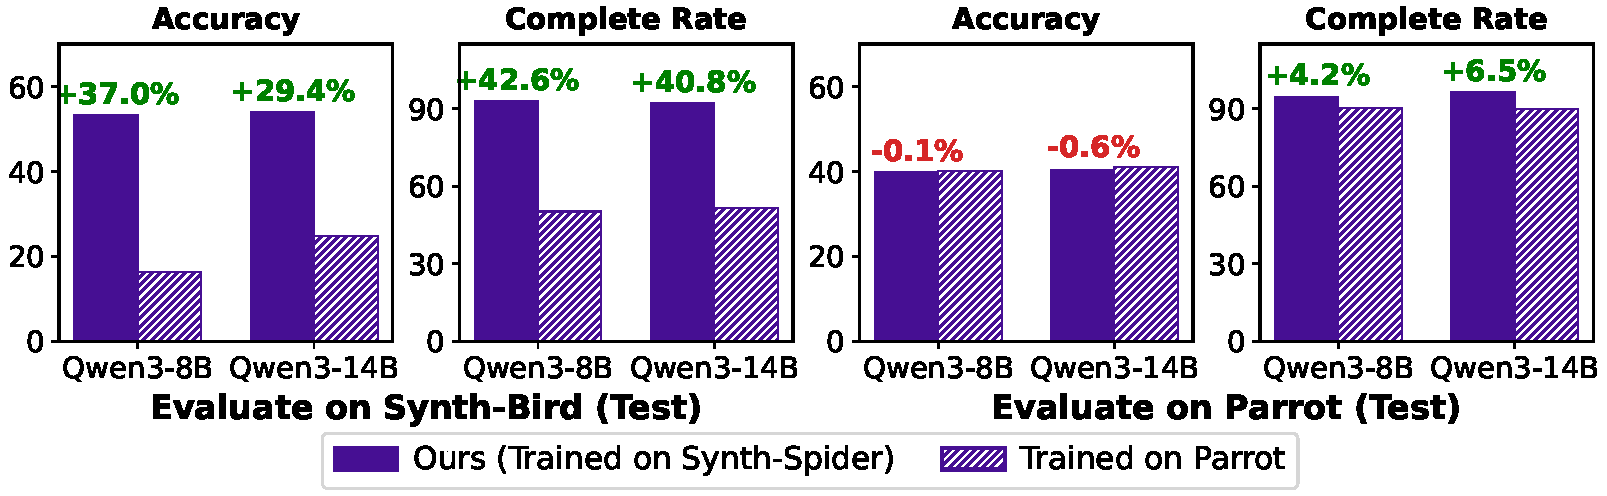
\includegraphics[width=1.01\columnwidth]{plots/plot/trained_on_spider_and_parrot.pdf}
    \vspace{-2em} 
    \caption{Evaluation results of models trained on Synth-Spider (Train) and Parrot (Train).}
    \label{\labelprefix fig:trained_on_spider_and_parrot}
    \vspace{-1em}
\end{figure}

% To further validate that a broader operator coverage and more diverse operator distribution are advantages of our synthesized dataset, we compare two models: one trained on Synth-Spider (Train) and the other trained on Parrot (Train), both evaluated on Parrot (Test). 
% As shown in the right part of Figure~\ref{fig:trained_on_spider_and_parrot}, the model trained on Synth-Spider achieves comparable accuracy to the model trained on Parrot (40.44 vs.\ 40.99 on Qwen3-14B), while obtaining a higher completion rate (96.41\% vs.\ 89.89\%). 
% This suggests that Synth-Spider's more diverse operator distribution exposes the model to a richer set of operator compositions during training, leading to stronger exploration capability and higher completion rates even on an out-of-domain test set.


\begin{shaded}
{
\stitle{R1D5:} The paper would be strengthened by discussing the limitations with a dedicated analysis of real-world failure cases.
}
\end{shaded}

\begin{figure}[t]
    \centering
    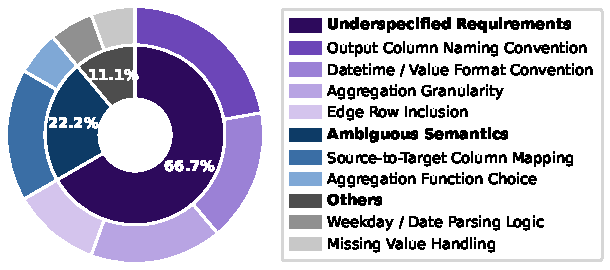
\includegraphics[width=1.01\columnwidth]{plots/plot/error_analysis_pie.pdf}
    \vspace{-2em} 
    \caption{Error analysis on Buildings.}
    \label{\labelprefix fig:error_analysis_pie}
    \vspace{-1em}
\end{figure}

\noindent{\bf RESPONSE}:
To better understand the limitations of \sys in realistic settings, we have \textbf{conducted a failure-case analysis on the Buildings dataset}, which consists of real-world ADP tasks. We added a new experiment, \textbf{Exp-\ref{exp:building_exp}}, in Section~\ref{subsec:in_depth_analysis}.

As summarized in Figure~\ref{\labelprefix fig:error_analysis_pie}, most failures can be attributed to the following two key challenges commonly encountered in real-world data preparation.

%
%To understand the limitations of our approach, we \textbf{conduct a dedicated analysis of failure cases} on the Buildings benchmark, which reflects real-world ADP scenarios. 
%We have added a new experiment \textbf{Exp-\ref{exp:building_exp} in Section~\ref{subsec:in_depth_analysis}}.
%As illustrated in Figure~\ref{\labelprefix fig:error_analysis_pie}, the real-world data preparation introduces two challenges.

\stitle{Ambiguous Column Semantics.}
In synthesized benchmarks, column names are typically self-descriptive (e.g., ``\textit{movie-title}'', ``\textit{release-year}''), making source-to-target mappings relatively straightforward. In contrast, real-world datasets often contain abbreviated or domain-specific column names (e.g., ``\texttt{hdd}'', ``\texttt{cdd}''), and the same concept may be represented differently across tables. This ambiguity leads to \emph{semantic column mapping errors}, which account for approximately 50\% of all failures. For example, a source column ``\texttt{hdd}'' (heating degree days) may need to be transformed into a target column \textit{heating-demand}, but the semantic relationship is difficult to infer from the column name alone.

%\stitle{Ambiguous Column Semantics.}
%In synthesized benchmarks, column names are typically self-descriptive (e.g., \textit{movie-title}, \textit{release-year}), making the mapping between source and target columns relatively straightforward. In real-world datasets, however, column names are often abbreviated or domain-specific (e.g., \texttt{hdd}, \textit{cdd}), and the same concept may be represented by different names across tables. This ambiguity directly causes the most common failure pattern named semantic column mapping errors (50\% of failures), where the model cannot correctly determine which source columns should be mapped or aggregated into which target columns. For instance, a source column named \textit{hdd} (heating degree days) needs to be aggregated into a target column named \textit{heating-demand}, but the model cannot infer this mapping because the abbreviation is domain-specific and the semantic connection is not evident from the column name alone.

\stitle{Underspecified Data Preparation Requirements.}
Another major challenge is that real-world target specifications are often incomplete. Unlike synthesized benchmarks, which explicitly define target schemas and transformation objectives, real-world tasks frequently describe desired outputs only at a high level. Important details, such as aggregation granularity (e.g., daily versus monthly) or aggregation semantics (e.g., sum versus average), may be omitted. As a result, \sys may generate incorrect grouping strategies or aggregation functions, leading to \emph{granularity mismatch errors} (22\% of failures) and \emph{domain logic errors} (11\% of failures).

%\stitle{Underspecified Data Preparation Requirements.}
%Synthesized benchmarks provide clear target schema descriptions that implicitly define the required granularity and aggregation logic. In real-world scenarios, the target specification is often under-specified. It may describe the desired output at a high level without explicitly stating whether daily or monthly granularity is expected, or whether a column should be summed or averaged. This causes granularity mismatch errors (22\% of failures), where the model selects incorrect GroupBy dimensions, and domain logic errors (11\% of failures), where the model applies inappropriate aggregation functions due to the lack of explicit domain constraints.

These findings suggest that future work should focus on improving schema-aware reasoning under ambiguous semantics and incorporating mechanisms for resolving underspecified user requirements. Such capabilities are likely to be important for deploying autonomous data preparation systems in real-world environments.

%These findings suggest that improving schema-aware reasoning under ambiguous semantics and handling underspecified requirements are key directions for future work.

{We have revised \textbf{Section~\ref{subsec:in_depth_analysis}} and added an experiment \textbf{Exp-\ref{exp:building_exp}} to include the above failure-case analysis and discussion.} A complete version of the failure-case analysis can be found in \textbf{Appendix~\ref{subsec:appendix_error_analysis}} of our technical report~\cite{technical_report}.